\cptr{Determining informative priors for cognitive models}
{Cognitive model priors}
{Michael D.\ Lee and Wolf Vanpaemel}

\newcommand{\GG}[1]{} % for the Jones and Dzhafarov order (see http://tex.stackexchange.com/questions/190842/same-author-same-year-bibliography-order)

\section{Introduction}

One way to think of cognitive modeling is as a natural extension of data analysis. Both involve developing, testing, and using formal models as accounts of brain and behavioral data. The key difference is the interpretation of the model likelihood and parameters. Data analysis typically relies on a standard set of statistical models, especially Generalized Linear Models (GLMs) that form the foundations of regression and the analysis of variance. In these models, parameters have generic interpretations, like locations and scales. Cognitive models, in contrast, aim to afford more substantive interpretations. It is natural to interpret the parameters in cognitive models as psychological variables like memory capacities, attention weights, or learning rates.

For both data-analytic and cognitive models, the likelihood is the function that gives the probability of observed data for a given set of parameter values. For data-analytic models, these likelihoods typically follow from GLMs. Cognitive models often use likelihoods designed to formalize assumptions about psychological processes, such as the encoding of a stimulus in memory, or the termination of search in decision making. Even when a cognitive model uses a likelihood function consistent with GLMs---for example, modeling choice probabilities as weighted linear combinations of stimulus attributes---it is natural to interpret the likelihood as corresponding to cognitive processes, because of the psychological interpretability of the parameters.

Their more elaborate interpretation means that cognitive models aim to formalize and use richer information and assumptions than data-analytic models do. In the standard frequentist approach, assumptions can only be used to specify the likelihood, and, less commonly, the bounds of the parameter space. The Bayesian approach offers the additional possibility of expressing assumptions in the prior distribution over the parameters. These prior distributions are representations of the relative probability that a parameter---or more generally, sets of parameters---have specific values, and thus formalize what is known and unknown about psychological variables.

Conceived in this way, priors are clearly an advantage of the Bayesian approach. They provide a way of formalizing available information and making theoretical assumptions, enabling the evaluation of the assumptions by empirical evidence, and applying what is learned to make more complete model-based inferences and predictions. Priors are often, however, maligned by those resistant to Bayesian methods \cite<e.g.,>{Edwards1991,Trafimow2005}. Even those who advocate Bayesian methods in cognitive modeling sometimes regard the need to specify a prior as a cost that must be borne to reap the benefits of complete and coherent inference. This lack of interest in the prior often results in what \citeA{Gill2014} terms ``Bayesians of convenience", who use priors they label vague, flat, non-committal, weakly informative, default, diffuse, or something else found nearby in a thesaurus. 

We believe failing to give sufficient attention to specifying priors is unfortunate, and potentially limits what cognitive modeling can achieve. Our view is that priors should be informative, which means that they should capture the relevant theoretical, logical, and empirical information about the psychological variables they represent \cite{Dienes2014,VanpaemelLee2012}. Only when modelers genuinely have no information about their parameters should informative priors be vague. In the usual and desirable situation in which something is known about parameters, assuming a vague prior loses useful information. The problem is put most emphatically by Jeff Gill (personal communication, August 2015):
\begin{quote}
``Prior information is all over the place in the social sciences. I really don't want to read a paper by authors who didn't know \emph{anything} about their topic before they started."
\end{quote}

Modelers do not strive to make likelihoods vague, but aim to make them consistent with theory, empirical regularities, and other relevant information. Since, in the Bayesian approach, priors and likelihoods combine to form the predictive distribution over data that \emph{is} the model, priors should also aim to be informative. It seems ironic to make the effort of developing a likelihood that is as informative as possible, only to dilute the predictions of the model by choosing a prior of convenience that ignores relevant theory, data, and logic. A worked example from psychophysics, showing how the unthinking assumption of vague priors can undo the theoretical content of a likelihood, is provided by \cite[see especially Figures~9 and 11]{Lee2016Stevens}.

There are probably two reasons for the routine use of vague priors, and the lack of effort in specifying informative priors. One involves discomfort with the fact that the choice of different informative priors will affect inference. These sorts of concerns about subjectivity are easy to dismiss. One reaction is to point out that it would be non-sensical if modeling assumptions like priors did not affect inference. A more constructive way to address the concern is to point out that developing likelihoods is just as challenging as developing priors, and inference is also sensitive to choices about likelihoods. Proposing models is a creative scientific act that, in a Bayesian approach, extends to include both priors and likelihoods. The sort of attitudes and practices modelers have in developing, justifying, and testing likelihoods should naturally carry over to priors. \citeA[p.37]{Leamer1983} insightfully highlights that both the likelihood and the prior are assumptions, and that a perceived difference in their subjectivity simply reflects the frequency of their use:
\begin{quote}
``The difference between a fact and an opinion for purposes of decision making and inference is that when I use opinions, I get uncomfortable. I am not too uncomfortable with the opinion that error terms are normally distributed because most econometricians make use of that assumption. This observation has deluded me into thinking that the opinion that error terms are normal may be a fact, when I know deep inside that normal distributions are actually used only for convenience. In contrast, I am \emph{quite} uncomfortable using a prior distribution, mostly I suspect because hardly anyone uses them. If convenient prior distributions were used as often as convenient sampling distributions, I suspect that I could be as easily deluded into thinking that prior distributions are facts as I have been into thinking that sampling distributions are facts.''
\end{quote} 

The second probable reason for the reliance on vague priors involves a lack of established methods for determining informative priors. Against this concern, the goal of this paper is to discuss how informative priors can be developed for cognitive models so that they are reasonable, useful, and capture as much information as possible. We identify several sources of information that can help to specify priors for cognitive models, and then discuss some of the methods by which this information can be incorporated into formal priors within a model. Finally, we identify a number of benefits arising from including informative priors in cognitive models. We mostly rely on published examples of the use of priors in cognitive modeling, but also point to under-used sources and methods that we believe provide important future directions for the field.
  
\section{Three illustrative cognitive models}

To help make some general and abstract ideas clear, we draw repeatedly upon three illustrative cognitive models, involving memory, categorization, and decision making. In this section, we describe these models in some detail.

\subsection{Exponential decay model of memory retention}

\begin{figure}[t]
\begin{center}
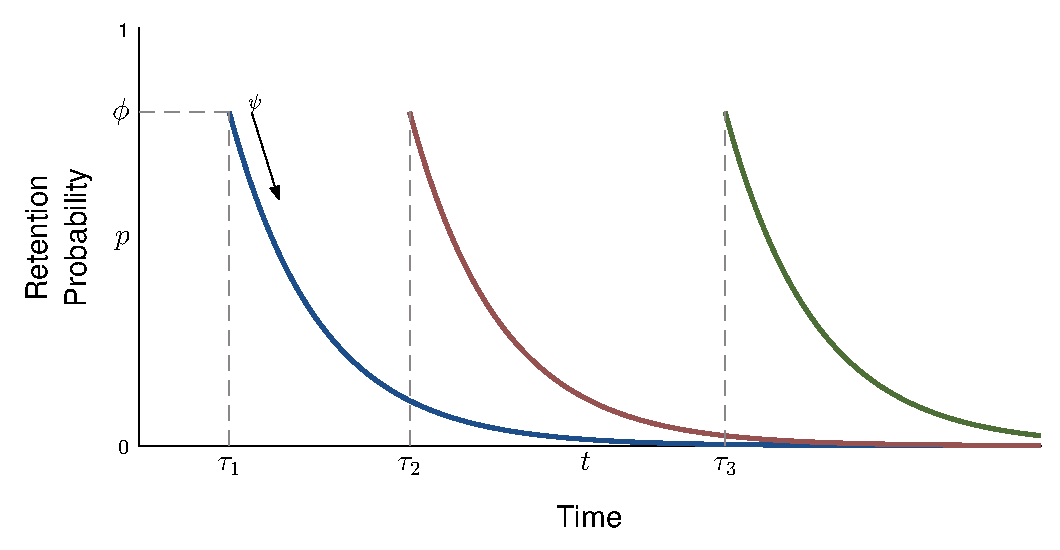
\epsfig{file=figs/ml1_Memory.eps,width=\columnwidth}
\caption{An exponential decay model of memory retention. The $x$-axis corresponds to time $t$, and the $y$-axis corresponds to the probability $p$ that an item will be recalled at a specified time. Retention curves for three items are shown. Each curve starts at the time the item was last rehearsed, corresponding to the parameters $\tau_1$, $\tau_2$, and $\tau_3$. The initial probability of recall at this time of last rehearsal is given by the parameter $\phi$. The rate of decrease in the probability of recall as time progresses depends on a decay parameter $\psi$.}
\label{Memory}
\end{center}
\end{figure}

A simple and standard model of memory retention assumes that the probability of recalling an item decays exponentially with time \cite{RubinWenzel1996}. One way to formalize this model is to assume that the probability of recalling the $i$th item at time $t_i$ if it was last studied at time $\tau_i$, is $p_i= \phi \exp\left\{-\psi \left(t_i-\tau_i\right)\right\}$. Figure~\ref{Memory} illustrates this model, showing the study times for three items, and the retention curves assumed by the model.

The $\phi$ parameter has the psychological interpretation of the initial probability of recall, that is, $\phi=p_i$ when $t_i=\tau_i$, while the $\psi$ parameter controls the rate at which recall probabilities change over time. The parameter space is restricted to $\psi>0$, so that the model formalizes the assumption of decay \cite<e.g.,>{Wickens1998}. The usual assumption is that the $\tau_i$ time intervals are known from the experimental design, based on explicit study presentations, or that all $\tau_i=0$ corresponding to the end of the study period. We consider a richer model in which the $\tau_i$ rehearsal times are treated as parameters, representing the last unobserved mental rehearsal of the item. This extension is made possible by the flexibility of Bayesian methods, and raises interesting questions about determining appropriate priors for the $\tau_i$ latent rehearsal parameters. 

\subsection{Generalized Context Model of categorization}

\begin{figure}[t]
\begin{center}
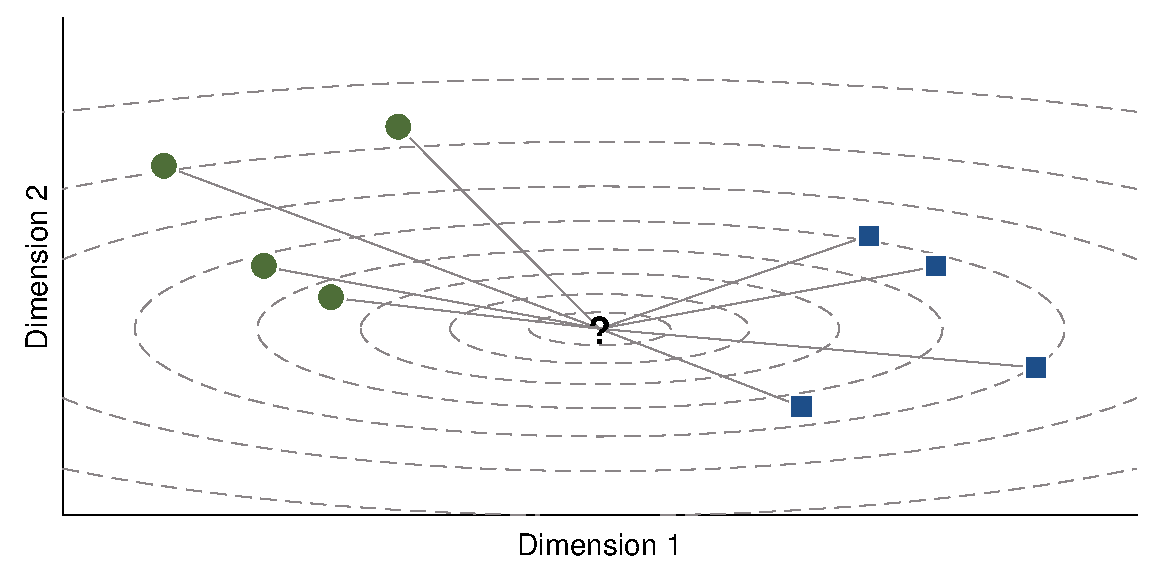
\epsfig{file=figs/ml1_Categorization.eps,width=\columnwidth}
\caption{The Generalized Context Model of categorization. Eight stimuli are shown in an attention-weighted two-dimensional representation. Four stimuli in one category are represented by circles, and four stimuli in an alternative category are represented by squares. More attention is given to the first stimulus dimension than to the second stimulus dimension, which ``stretches" the space to emphasize differences between the stimuli on the first dimension. Generalization gradients from the stimulus to be categorized, marked by ``?", to the known stimuli are shown by ellipses. These gradients produce measures of similarity between the stimuli, based on their distance in the space, and the steepness of the generalization gradient. The total similarity between the stimulus to be categorized and the known exemplars determines, together with response determinism and category bias,  the categorization response probabilities.}
\label{Categorization}
\end{center}
\end{figure}

The Generalized Context Model \cite<GCM:>{Nosofsky1986} is a seminal model of categorization. It assumes that categorization behavior is based on comparing the attention-weighted similarity of a presented stimulus to known exemplars of the possible alternative categories. A visual representation of the core assumptions of the model is provided in Figure~\ref{Categorization}. This figure shows, in an attention-weighted psychological space, the generalization gradients of similarity for a new stimulus ``?" into two categories represented by circle and square exemplars.

Formally, in the version of the GCM that we consider, the $i$th stimulus is represented by the coordinate location $\bm x_i$, so that the attention-weighted distance between the $i$th and $j$th stimuli is $d_{ij} = \sum_{k}\omega_k \left|x_{ik}-x_{jk}\right|$, where $\omega_k$ is the attention given to the $k$th dimension. Accordingly, a dimension receiving more attention will be more influential in determining distances than the ones receiving less attention. The similarity between these stimuli is then $s_{ij} = \exp\left(-\lambda d_{ij}\right)$, with $\lambda$ controlling the generalization gradient between stimuli. The similarity of the $i$th stimulus to category A is the sum of the similarities to all the stimuli in the category: $s_{iA} = \sum_{j \in A} s_{ij}$. Finally, the probability of a category response placing the $i$th stimulus in category A is $p_{iA}=\beta_A s_{iA}^\gamma/\sum_C \beta_C s_{iC}^\gamma$, where the index $C$ is across all possible categories, $\beta_C$ is a response bias to category C, and $\gamma$ controls the extent to which responding is deterministic or probabilistic, with higher values corresponding to more determinism.

\subsection{Wiener diffusion model of decision making}

Sequential sampling models of decision making assume that evidence is gathered from a stimulus over time until enough has been gathered to make a choice \cite{Luce1986}. The Weiner diffusion model \cite{RatcliffMcKoon2008} model is a simple, but widely used, sequential sampling model for two-choice decisions. It assumes evidence takes the form of samples from a Gaussian distribution with mean $\nu$. Total evidence starts at $\theta$ and is summed until it reaches a lower bound of zero or an upper bound of $\alpha$. The decision made corresponds to the boundary reached, and the response time is proportional to the number of samples, with the inclusion of an additive offset $\delta$.

\begin{figure}[tp]
\begin{center}
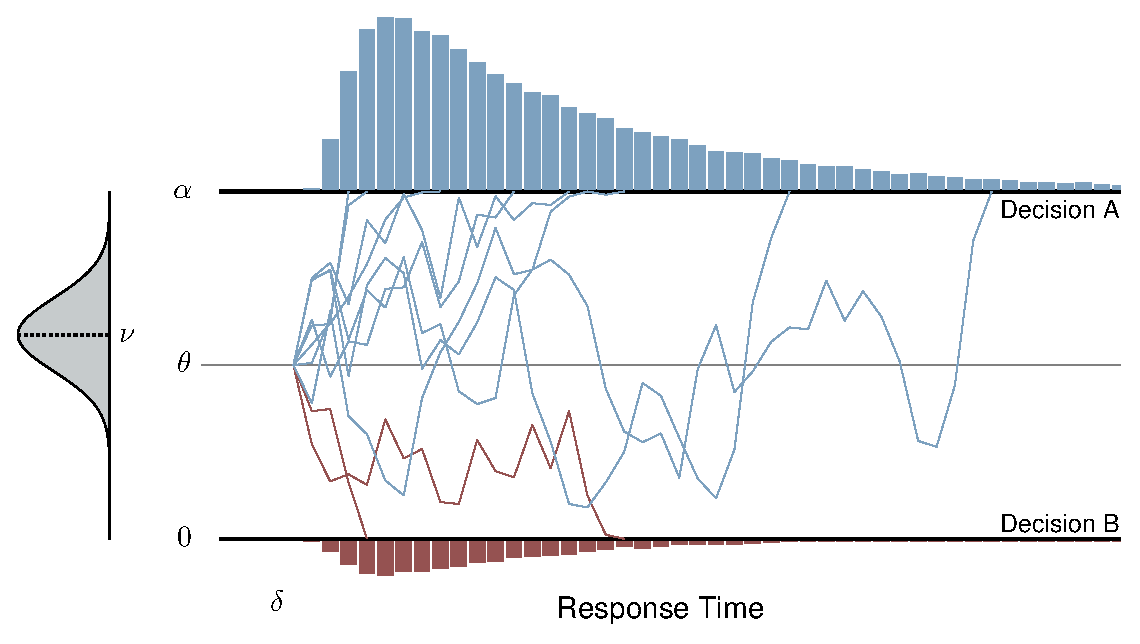
\epsfig{file=figs/ml1_DecisionMaking.eps,width=\columnwidth}
\caption{The Wiener diffusion model of decision making. A two-choice decision about a stimulus is made by sampling repeatedly from an evidence distribution for the stimulus, represented by a Gaussian distribution with mean $\nu$. The samples are combined to form an evidence path, and a number of illustrative sample paths are shown. These paths start from an initial evidence value $\theta$, and continue until they reach an upper bound of $\alpha$ or a lower bound of $0$. The decision made corresponds to which boundary is reached. The response time is proportional to the number of samples collected, plus a constant $\delta$ representing the additional time needed to encode the stimuli and execute the response behavior. The decision and response time behavior is shown by the histograms above and below the decision boundaries. The histogram at each boundary is proportional to the response time distribution for that decision, and the area under each distribution represents the overall probability of that decision.}
\label{DecisionMaking}
\end{center}
\end{figure}

The decision model is shown Figure~\ref{DecisionMaking}. The stimulus provides evidence favoring decision A, because the mean $\nu$ of the Gaussian characterizing the evidence is greater than zero. The decision and response times are shown by the histograms at each boundary. The shape of the histogram represents the response time distribution for each type of decision, and the area under each distribution represents the probability of each decision. It is clear that decision A is more likely, and both response time distributions have a characteristic non-monotonic shape with a long-tailed positive skew.

The $\nu$ parameter, usually called the drift rate, corresponds to the informativeness of the stimulus. Larger absolute values of $\nu$ correspond to stimuli that provide stronger evidence in favor of one or other of the decisions. Smaller absolute values of $\nu$ correspond to less informative stimuli, with $\nu=0$ representing a stimulus that provides no overall information about which decision to make.
 
Figure~\ref{DecisionMaking} also shows a number of sample paths of evidence accumulation. All of the paths begin at the starting point $\theta$, which is half-way between the boundaries at $\theta = \alpha/2$. Other starting points would favor one or other decision. The starting point parameter $\theta$ can theoretically be conceived as a bias in favor of one of the decisions. Such a bias could arise, psychologically, from prior evidence in favor of a decision, or as a way of incorporating utilities for correct and incorrect decisions of each type.

The $\alpha$ parameter, usually called boundary separation, corresponds to the caution used to make a decision, as manipulated, for example, by speed or accuracy instructions. Larger values of $\alpha$ lead to slower and more accurate decisions, while smaller values lead to faster but more error-prone decisions.

Finally, the offset $\delta$ corresponds to the component of the response time not accounted for by the sequential sampling process, such as the time taken to encode the stimulus and produce motor movements for a response. It is shown in Figure~\ref{DecisionMaking} as an offset at the beginning of the evidence sampling process, but could also be conceived as having two components, with an encoding part at the beginning, and a responding part at the end.

\section{Sources for determining informative priors}

In this section, we identify several sources of information that can be used in determining priors, and explain how these relate to the meaningful parameters of the three illustrative cognitive models.

\subsection{Psychological and other scientific theory}

The most important source of information for specifying priors in cognitive models is psychological theory. In cognitive modeling, likelihood functions largely reflect theoretical assumptions about cognitive processes. The exponential decay memory retention model commits to the way in which information is lost over time, assuming, in part, that the rate of this loss is greatest immediately after information is acquired. The categorization model commits to assumptions of exemplar representation, selective attention, and similarity comparisons in categorization. The decision model commits to the sequential sampling of information from a stimulus until a threshold level of evidence is reached. These assumptions are the cornerstones on which the likelihood functions of the models are founded. Analogously, theoretical assumptions about psychological variables should be the cornerstones on which priors are determined \cite{Vanpaemel2009,Vanpaemel2010}. Ideally, psychological theories should make assumptions about not just psychological processes, but also about the psychological variables that control those processes, leading to theory-informed priors.

One possibility is that theoretical assumptions dictate that some parameter values are impossible, consistent with the non-Bayesian restriction of the parameter space. In the memory retention model, the theoretical assumption that the probability of recall decreases over time constrains the memory retention parameter $\psi > 0$. In the categorization model, the theoretical assumption that generalization gradients decrease as stimuli become less similar, constrains the parameter $\lambda \geq 0$ \cite{Nosofsky1986,Shepard1987}. 

Other sorts of theorizing can provide more elaborate information about possible combinations of values for a set of parameters. Theories of attention, for example, often assume it is a capacity-limited resource. In the categorization model, this constraint is usually implemented as $\sum_k \omega_k =1$, so that the values of the attention parameters collectively meet a capacity bound. In effect, the theoretical assumption still dictates that some parameter values are impossible, but now the constraint applies jointly to a set of parameters.

As theories become more general and complete they can provide richer information. Theory can provide information beyond which values are possible, and indicate which values are probable. The optimal-attention hypothesis \cite{Nosofsky1986} assumes that people distribute their attention near optimally in learning a category structure for a set of stimuli. This assumption implies that values of the $\omega_k$ parameters that maximally separate the stimuli in each category from each other are expected. For example, in Figure~\ref{Categorization}, the stimuli in the two different categories vary more along the first than the second dimension. The optimal-attention hypothesis thus assumes that attention will be given to the first dimension to a level $\omega_1$ somewhere near 1 that maximally distinguishes the two categories.

The optimality principle underlying the optimal-attention hypothesis could be extended to other cognitive models and phenomena. The principle that the most likely values of a parameter are those that maximize some aspect of behavioral performance is a generally applicable one. Optimality could be a fundamental source for setting priors in cognitive process models, but is currently under-used. Embedding the optimality principle within cognitive process models through priors would bring these models in closer contact with the successful rational models of cognition, where optimal behavior is a core theoretical assumption \cite<e.g.,>{Anderson1992,ChaterEtAl2006,TenenbaumEtAl2011}.

A different example of using theory to develop a prior is provided by \citeA{RouderEtAl2007}, who propose a mass-at-chance model for performance in subliminal priming tasks. Their theoretical expectations are that some people will perform at chance, but others will use a threshold-based detection process to perform above chance. \citeA[see especially their Figure 3]{RouderEtAl2007} consider different theoretical possibilities about the distribution of detection probabilities for people performing above chance. One possibility is that all detection probabilities are equally likely, so that it is constrained between $\frac{1}{2}$ and 1. Another possibility is that they are only slightly above chance, so that, for example, few people are expected to have a detection probability higher than (say) 70\%. A third possibility is that people who are not at chance all have perfect accuracy, so that there are only two possible detection probabilities, $\frac{1}{2}$ and $1$. \citeA{RouderEtAl2007} consider only the first two options to be reasonable, and express this theoretical assumption by constraining a variance parameter to be smaller than 1. In this way, \citeA{RouderEtAl2007} establish a direct link between substantive theoretical assumptions about the nature of people's performance on the task and an exact range constraint on a variance parameter.

In some modeling situations, the likelihood can carry little theoretical content, and the theoretically most-relevant information is about the parameters. One example is provided by \citeA{Lee2016}, in a Bayesian implementation of a model originally developed by \citeA{HilbigMoshagen2014}, for inferring which of a number of decision strategies people used in a cue-based decision-making task. The likelihood function is made up of simple binomial distributions, corresponding to how often an alternative is chosen for the trials within each decision type. Because different strategies predict different choice patterns, all of the important theoretical content is reflected in constraints on the choice parameters within the binomial distributions. For example, the new strategy introduced by \citeA{HilbigMoshagen2014} assumes an ordering for the probability of choice of different types of questions, and this information is represented by order constraints on the parameters corresponding to these probabilities in a joint prior. A similar earlier example in which the prior is theoretically more important than the likelihood is provided by \citeA{MyungEtAl2005}, who use order constraints on the parameters representing probabilities, to formalize several decision-making axioms such as the monotonicity of joint receipt axiom and the stochastic transitivity axiom.

Finally, we note that sciences other than psychology can and should provide relevant theoretical information. Physics, for example, provides the strong constraint---unless the controversial assumption of the existence of extra-sensory perception is made---that an item in a memory task cannot be rehearsed before it has been presented. This means, in the memory model, that each $\tau_i$ rehearsal parameter is constrained not to come before the actual time $t_i$ the item was presented, so that $\tau_i \geq t_i$. Another example of the potential relevance of multiple other scientific fields to determine priors is provided by the offset parameter $\delta$ in the decision model. Neurobiological and chemical processes, such as the time taken for physical stimulus information to transmit through the brain regions responsible for low-level visual processing, should constrain the component of this parameter that corresponds to the time needed to encode stimuli. Physiological theories specifying, for example, distributions of the speeds of sequences of motor movements, should constrain the component of the parameter that corresponds to the time taken to produce an overt response. Thus, a theoretically meaningful prior for $\delta$ in the decision model could potentially be determined almost entirely by theories from scientific fields outside cognitive psychology. 

\subsection{Logic and invariances} 

The meaning of parameters can have logical implications for their prior distribution. Logic can dictate, for example, that some values of a parameter are impossible \cite{Taagepera2007}. Probabilities are logically constrained to be between 0 and 1, and variances and other scale parameters are constrained to be positive. In the memory and decision models, the probability parameters $\phi$, $\beta$, and $\theta$ are both logically constrained to be between 0 and 1. 

The nature of a modeling problem can also provide logical constraints. The decision model has no meaning unless the starting point $\theta$ is between 0 and the boundary $\alpha$, and has the same substantive interpretation under the transformation $\left(\alpha,\theta\right)\rightarrow\left(-\alpha,-\theta\right)$ that ``flips'' the boundary and starting point below zero. This invariance leads to the constraints $\alpha,\ \theta > 0$ and $0 < \theta < \alpha$ to make the model meaningful.

In general, superficial changes to a modeling problem that leave the basic problem unchanged should not affect inference, and priors must be consistent with this. In our memory and decision models, for example, inferences should not depend on whether time is measured in seconds of milliseconds, and the way priors over $\left(\phi,\psi,\tau\right)$ and $\left(\alpha,\theta,\nu,\delta\right)$ are determined should lead to the same results regardless of the unit of measurement. This is a specific example of the general principle of transformation invariance, which requires that priors lead to the same result under transformations of a problem that change its surface form, but leave the fundamental problem itself unchanged \cite{LeeWagenmakers2005}. In the time scale example, the transformation is scalar multiplication of a measurement scale. In general, the transformation can involve much more elaborate and abstract manipulations of the inference problem being posed, as in Jaynes' \citeyear[Ch. 12]{Jaynes2003} discussion of a famous problem in statistics known as Bertrand's paradox. The problem involves the probability of randomly thrown sticks intersecting a circle and is notorious for having different reasonable priors lead to different inferences. By considering logical rotation, translation, and dilation invariances for the circle, inherent in the statement of the problem, it is possible to determine an appropriate and unique prior. Motivated by these sorts of examples, we think that transformation invariance is a potentially important principle for determining priors. It is difficult, however, to find examples in cognitive modeling, and we believe more effort should be devoted to exploring the possibilities of this approach.

\subsection{Previous data and modeling} 

Cognitive psychology has a long history as an empirical science, and has accumulated a wealth of behavioral data. Empirical regularities for basic cognitive phenomena are often well established. These regularities provide an accessible and substantial source of information for constructing priors. For example, response time distributions typically have a positive skew \cite<e.g.,>{Luce1986} and people often probability match in categorization, which means their probability of choosing each alternative is given by the relative evidence for that alternative \cite{ShanksEtAl2002}. This last observation is a good example of how empirical regularities can help determine a prior, and is applicable to the $\gamma$ parameter in the categorization model. Different values of this parameter correspond to different assumptions about how people convert evidence for response alternatives into a single choice response. When $\gamma=1$, decisions are made by probability matching. As $\gamma$ increases above one, decision making becomes progressively more deterministic in choosing the alternative with the most evidence. As $\gamma$ decreases below one, the evidence plays a lesser role in guiding the choice until, when $\gamma=0$, choices are made at random. Thus, previous empirical findings that provide evidence as to whether people respond deterministically, probability match, and so on, can naturally provide useful information for determining a data-informed prior over the $\gamma$ parameter \cite<e.g.,>{LeeEtAl2015}.

Cognitive psychology is also a model-based science, and so there are many reported applications of models to data. These efforts provide inferences about parameters that can inform the development of priors. For each of the memory, categorization, and decision models, there are many published relevant applications to data, including inferred parameter values \cite<e.g.,>{Nosofsky1991b,RatcliffSmith2004,RubinWenzel1996}. The approach of relying on previous parameter inferences to determine priors for related models is becoming more frequent in cognitive modeling. Some recent examples include \citeA{GuEtAl2016} in psychophysics, \citeA{Gershman2016} in reinforcement learning models, \citeA{Vincent2015} in the context of temporal discounting, \citeA{WiehlerEtAl2015} for different clinical sub-populations in the context of gambling, and \citeA{DonkinEtAl2015a} in the context of a visual working memory model. In an interesting application of the latter model, \citeA{KaryEtAl2015} used vague priors for key parameters, and used the data from the first half of their participants to derive the posterior distributions. These posteriors were subsequently used as a basis for  priors in the analysis of the data from the remaining half of the participants.

\subsection{Elicitation}

There is a reasonably well-developed literature on methods designed to elicit priors from people \cite<e.g.,>{AlbertEtAl2012,GarthwaiteEtAl2005,KadaneWolfson1998,OHaganEtAl2005}. These methods are used quite extensively in modeling in some empirical sciences, but do not seem to be used routinely in cognitive modeling. Elicitation methods are designed to collect judgments from people---often with a focus on experts---that allow inferences about a probability distribution over unknown quantities. The most common general approach involves asking for estimates of properties of the required distribution. This can be as simple as asking for a minimum and maximum possible value, or the bounds on (say) an 80\% credible interval for an observed quantity.

These elicitation methods can ask directly about latent parameters of interest, or about predicted observable quantities implied by values of those parameters. Obviously, when elicitation focuses on quantities related to the parameters, rather than the parameters themselves, a model is needed to relate people's judgments to the desired probability distributions. For example, in a signal detection theory setting, it is possible to elicit distributions for discriminability and bias parameters directly, or infer them from elicited hit and false-alarm rates based on a standard model. The logical end-point of asking about quantities implied by parameters is to ask about idealized data \cite{Winkler1967}. This is a potentially very useful approach, because often experts can express their understanding most precisely and accurately in terms of data. \citeA{Kruschke2013} provides a good example of this approach for data-analytic models in psychology, and it is clear it generalizes naturally to cognitive models.

Another approach to constructing elicitation-based priors used in applied settings require a series of judgments between discrete options, from which a probability distribution representing uncertainty can be derived \cite<e.g.,>{WelshEtAl2004}. Along these lines, one potentially useful recent development is the elicitation procedure known as iterated learning \cite{KalishEtAl2007,LewandowskyEtAl2009}. This clever procedure requires a sequence of people to do a task, such as learning a category structure, or the functional relationship between variables. Each person's task depends on the answers provided by the previous person, in a way that successively amplifies the assumed common prior information, or inductive bias, people bring to the task. Applying this procedure to categorization, \citeA{CaniniEtAl2014} found that, when learning categories, people have a strong bias for a linear category boundary on a single dimension, provided that such a dimension can be identified. Translating this observation to the $\omega_k$ parameters in the categorization model implies that, in absence of any other information about category structures, these parameters are expected to be close to 0 or 1. It is a worthwhile topic for future research to find ways of formally translating this sort of information into a prior for a cognitive model. 

\section{Methods for determining informative priors}

The sources of information identified in the previous section are only pre-cursors to the complete formalization of a prior distribution. Knowing, for example, that some values of a parameter are theoretically impossible does not determine what distribution should be placed on the possible values. In this section, we identify some methods for taking relevant information, and using it to construct a formal prior distribution.

\subsection{Constraint satisfaction} 

If available information, whether by theoretical assumption, out of logical necessity, or from some other source, constrains parameter values, these constraints can be used as bounds. To determine the prior distribution within these bounds, the maximum-entropy principle provides a powerful and general approach (\citeNP[Ch. 11]{Jaynes2003}; \citeNP{Robert2007}). Conceptually, the idea of maximum entropy is to specify a prior distribution that satisfies the constraints, but is otherwise as uninformative as possible. In other words, the idea is for the prior to capture the available information, but no more. Common applications of this approach in cognitive modeling include setting uniform priors between 0 and 1 on probabilities, setting a form of inverse-gamma prior on variances \cite<see>[for discussion]{Gelman2006}, and enforcing order constraints between parameters \cite<e.g.,>{HoijtinkEtAl2008,Lee2016}.

\begin{figure}[tp]
\begin{center}
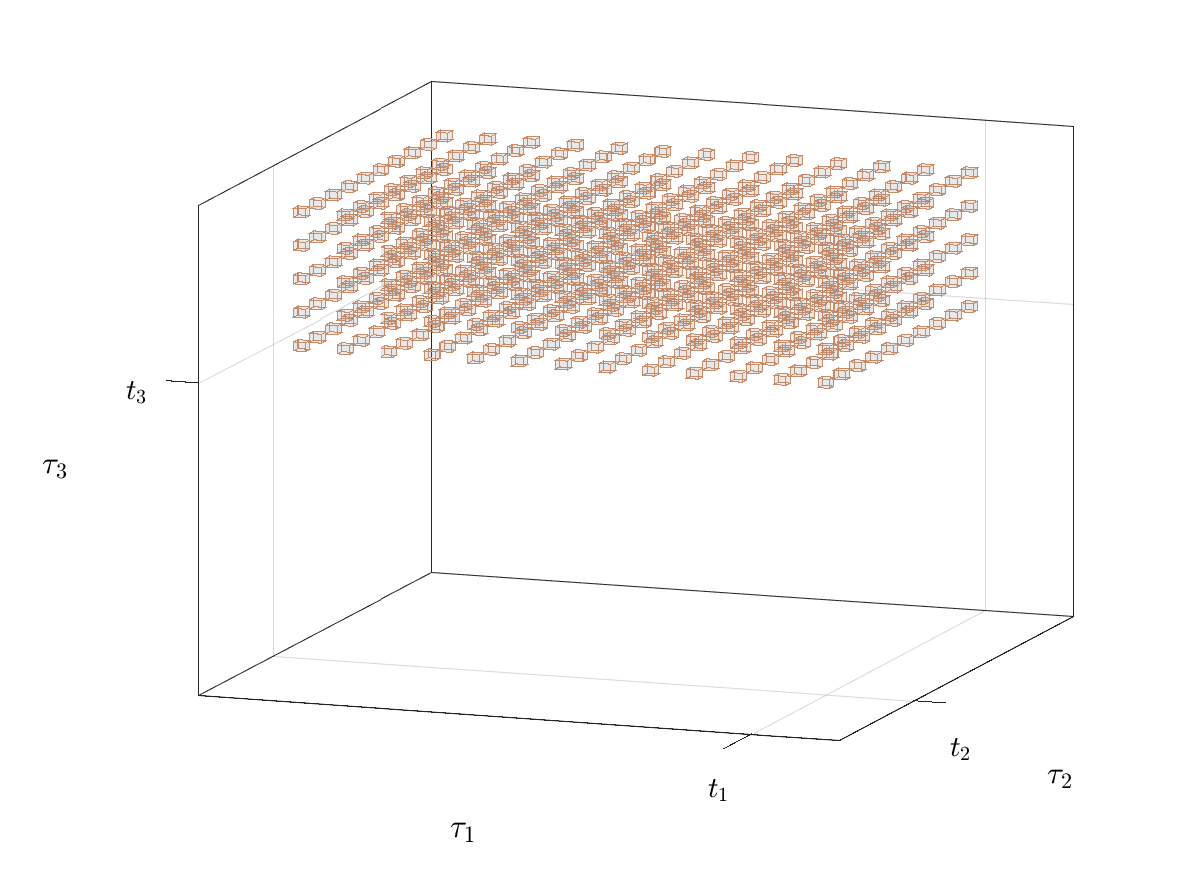
\epsfig{file=figs/ml1_Constraint.eps,width=\columnwidth}
\caption{A prior specified by constraint satisfaction for the memory retention model. The three axes correspond to the last rehearsal times of three studied items, represented by the model parameters $\tau_1$, $\tau_2$, and $\tau_3$. The case considered involves these items having been first presented at known times $t_1$, $t_2$, and $t_3$. The shaded region corresponds to the set of all possible rehearsal times $\left(\tau_1,\tau_2,\tau_3\right)$ that satisfy the logical constraint that an item can only be rehearsed after it is presented, so that $\tau_1\geq t_1$, $\tau_2\geq t_2$, and $\tau_3\geq t_3$. The uniform distribution of prior probability within this constraint satisfaction region follows from the maximum-entropy principle.}
\label{Constraint}
\end{center}
\end{figure}

A good example of applying the maximum-entropy principle to order constraints involves the $\tau_i$ rehearsal parameters in the memory model, if they are subject to the constraint that an item cannot be rehearsed before it has been presented. Figure~\ref{Constraint} shows the resultant joint prior on $\left(\tau_1,\tau_2,\tau_3\right)$ if the three study items are presented at times $t_1$, $t_2$, and $t_3$. Only rehearsal parameter combinations that are in the shaded cube have prior density. The uniformity of the prior in this region follows from the maximum-entropy principle, which ensures that it satisfies the known constraints about when the items could be rehearsed, but otherwise carries as little information as possible.

More general applications of the maximum-entropy principle are rare in the cognitive modeling literature. \citeA{VanpaemelLee2012} present an example that is conceptually close, relating to setting the prior on the attention-weight parameter $\omega$ in the categorization model. The prior is assumed to be a beta distribution, and the optimal-attention hypothesis is used to set the mode of the prior to the value that best separates the stimuli from the different categories. The optimal-attention hypothesis, however, is not precise enough to determine an exact shape for the prior, but the precision of the beta distribution could have been determined in a more principled way by maximum-entropy methods. This would have improved on the heuristic approach actually used by \citeA{VanpaemelLee2012} to set the precision. We think maximum-entropy methods are under-used, and that they are an approach cognitive modeling should adopt and develop, especially given the availability of general statistical results that relate known constraints to maximum-entropy distributions \cite<e.g.,>{LismanVanZuylen1972}.

\subsection{Prior prediction} 

By specifying a likelihood and a prior, it is possible to calculate the prior predictive distribution, which is a prediction about the relative probability of all possible data sets, based solely on modeling assumptions. If information is available about possible or plausible data patterns, most likely based on previously established empirical regularities or on elicitation, then one approach is to develop a prior distribution that leads to prior predictive distributions consistent with this information. A very similar approach is Parameter Space Partitioning \cite<PSP:>{PittEtAl2006}, which divides the entire parameter space into mutually exclusive regions that correspond to different qualitative data patterns a model can generate. Priors can then be determined by favoring those regions of the parameter space that generate data patterns consistent with expectations, and down-weighting or excluding regions corresponding to less plausible or implausible data patterns.

\begin{figure}[tp]
\begin{center}
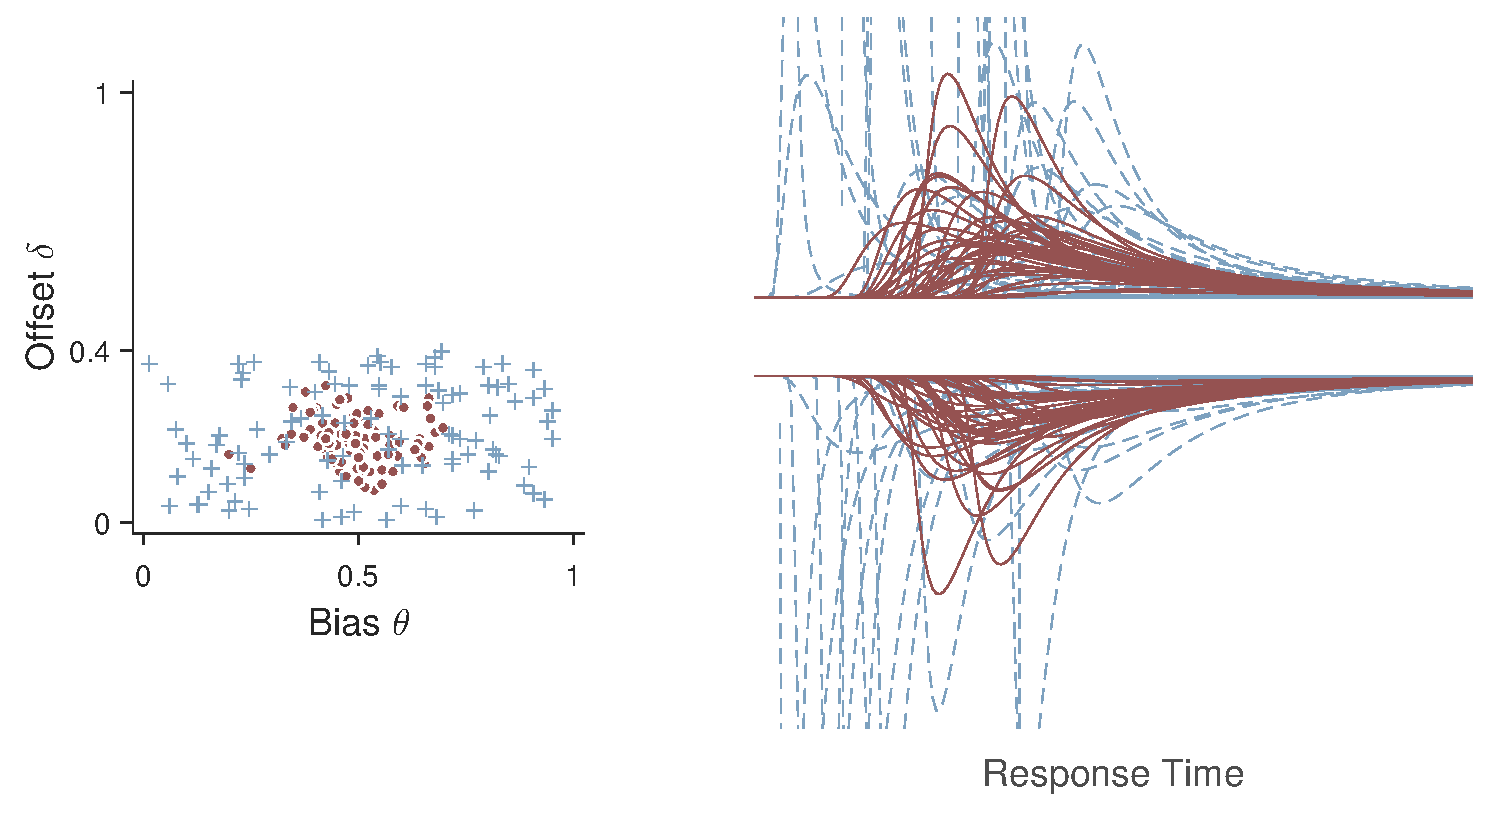
\epsfig{file=figs/ml1_PriorPredictionDiffusion.eps,width=\columnwidth}
\caption{Developing a prior distribution using prior prediction for the decision model. The left panel shows the joint parameter space for the bias $\theta$ and offset $\delta$ parameters. The right panel shows the joint decision and response time distributions generated by the model. Two specific prior distributions are considered, represented by circles and crosses in the parameter space, with corresponding solid and broken lines in the model space. The prior represented by the circles makes stronger assumptions about both bias and offset, and predicts a more reasonable set of response time distribution than the vaguer prior represented by the crosses.}
\label{PriorPrediction}
\end{center}
\end{figure}

A closely-related approach involves considering the predictions over psychologically meaningful components of a model that are implied by priors over their parameters. If information is available about the plausible form of these parts of models, most likely based on theory, it makes sense to define parameter priors that produce reasonable prior distributions for them. Figure~\ref{PriorPrediction} shows an example of this second approach using the decision model. Each combination of the starting point $\theta$ and offset $\delta$ parameters, which lie in the two-dimensional parameter space on the left, corresponds to a single joint decision and response time distribution for the two choices, shown on the right. Two different joint prior distributions over the parameters are considered. The first prior distribution, shown by circles in parameter space, has a truncated Gaussian prior for $\theta$ with a mean of 0.5 and a standard deviation of 0.1 in the valid range $0< \theta< 1$, and a truncated Gaussian prior for $\delta$ with a mean of 0.2 and a standard deviation of 0.05 in the valid range $\delta>0$. The second prior, shown by the crosses, simply uses uniform priors on reasonable ranges for the parameters: $0< \theta< 1$, and $0< \delta< 0.4$.

The consequences of these different assumptions are clear from the corresponding distributions shown in the model space, which shows response time distributions generated by the decision models corresponding to both priors, for the same assumptions about boundary separation and the distribution of drift rates. The predictions of the decision model with the first prior distribution, shown by solid lines, cover the sorts of possibilities that might be expected, in terms of their qualitative position and shape. The predictions for the second prior distribution, shown by broken lines, however, are much less reasonable. Many of the predicted response time distributions start too soon, and are too peaked. These weaknesses can be traced directly to the vague priors allowing starting points too close to the boundaries, and permitting very fast non-decision times. This analysis suggests that the sorts of assumptions about the starting point and offset made in forming the first prior may be good ones for the decision model. In this way, the relationship between prior distributions and psychologically interpretable components of the model provides a natural way to apply relevant knowledge in developing priors.

Using prior prediction to determine prior distributions in cognitive modeling is a general and relatively easy approach. Theorists often have clear expectations about model components like retention functions, generalization gradients, or the shapes of response time distributions, as well as about the data patterns that will be observed in specific experiments, which can be examined in prior predictive distributions. While it is currently hard to find cognitive modeling examples of priors being developed by the examination of prior predictions (see \citeNP{Lee2015JDM,LeeDanileiko2014}, for exceptions), we expect this state of affairs will change quickly. One reason for this optimism is that prior predictions are slowly starting to appear in the cognitive modeling literature, with goals that are closely related to setting priors. For example, \citeA{KaryEtAl2015} and \citeA{TurnerEtAl2013} examine the prior predictions of memory models, as a sanity check before application. In addition, prior predictive distributions have been used for assessing model complexity \cite{Vanpaemel2009}, for evaluating model falsifiability, and for testing a model against empirical data \cite{Vanpaemel2016b}. 

\subsection{Hierarchical extension}

An especially important method for developing priors in cognitive modeling involves extending the cognitive model itself. The basic idea is to extend the model so that priors on parameters are determined as the outcome of other parts of an extended model. This involves incorporating additional theoretical assumptions into the model, and is naturally achieved by hierarchical or multi-level model structures \cite{Lee2011,Vanpaemel2011}. None of the illustrative memory, categorization, or decision models, as we presented them, have this property, which is representative of the field as a whole. The parameters in these models represent psychological variables that initiate a data generating process, and so priors must be placed explicitly on these parameters. The key insight of the hierarchical approach is that these psychological variables do not exist in isolation in a complete cognitive system, but can be conceived as the outcomes of other cognitive processes. Including those other processes within a more complete model thus naturally defines a prior for the original parameters.

\begin{figure}[tp]
\begin{center}
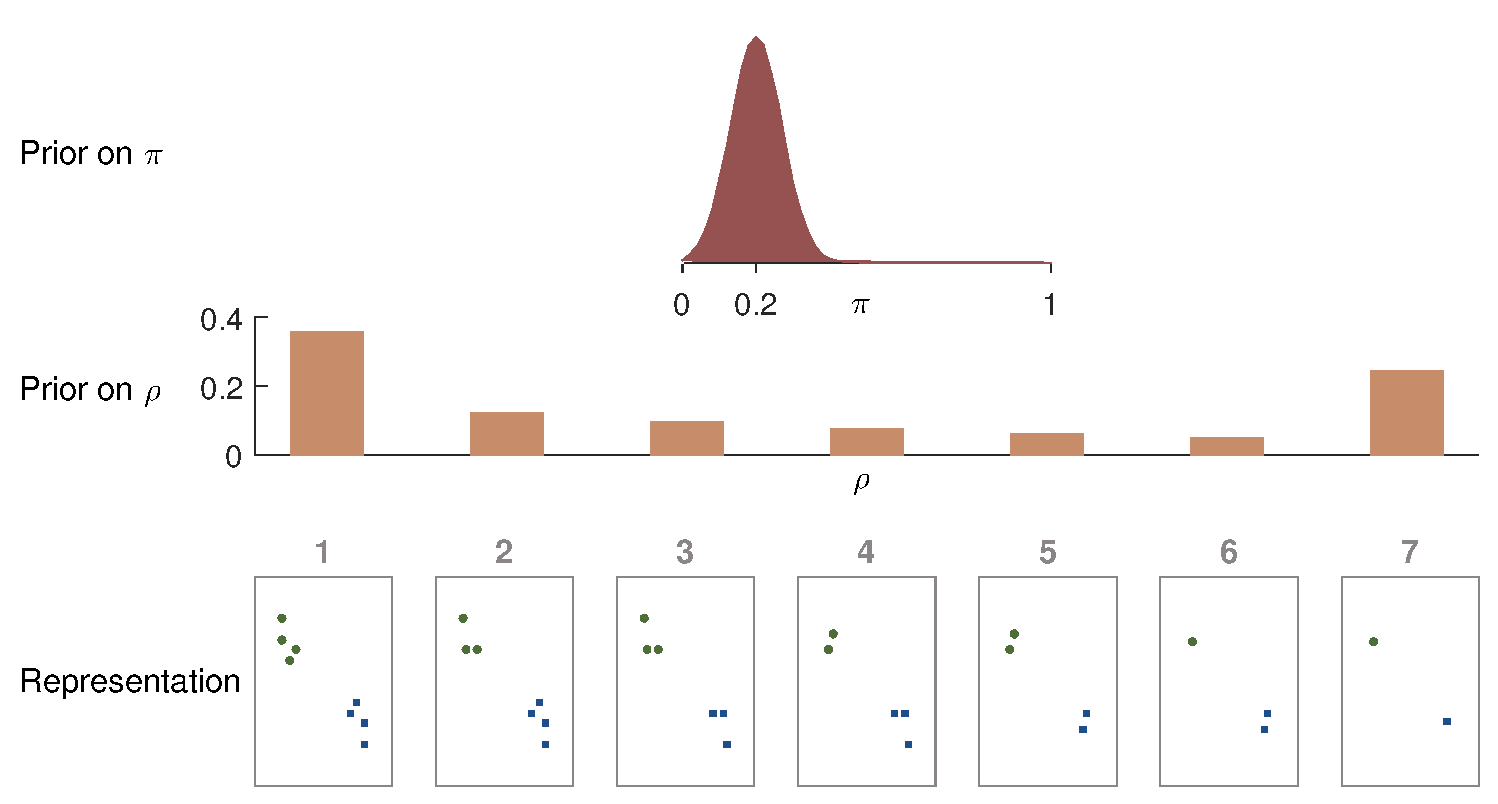
\epsfig{file=figs/ml1_Hierarchical.eps,width=\columnwidth}
\caption{A hierarchical approach to determining a prior distribution for the representation index parameter $\rho$ in an expanded version of the categorization model. The top panel shows an assumed prior distribution over a parameter $\pi$ that corresponds to the probability of merging a pair of stimuli in an exemplar representation. The bottom panels show a selection of 7 possible representations generated by this merging process, for a categorization problem with four stimuli in each of two categories, distinguished as circles and squares. The full exemplar representation is shown on the left, the prototype representation is shown on the right, and some of the representations with intermediate levels of abstraction are shown between. The bar graph in the middle panel shows the prior probability on the representational index parameter $\rho$ implied by the merging process and the prior distribution on $\pi$.}
\label{Hierarchical}
\end{center}
\end{figure}

 An example of this approach is provided by \citeA{LeeVanpaemel2008}, who focus on the Varying Abstraction Model \cite<VAM:>{VanpaemelStorms2008}. This model expands the categorization model by allowing for different sorts of category representations, ranging from an exemplar representation in which every stimulus in each category is represented, to a prototype representation in which each category is represented by a single summary point. Some of these possibilities are shown in the 7 bottom panels in Figure~\ref{Hierarchical}, for a case in which there are two categories with four stimuli each. The representation on the far left is the exemplar representation, as assumed by the original categorization model, while the representation on the far right is the prototype representation. The intermediate representations show different levels of abstraction, as the detail of exemplar representation gives way to summary representations of the categories. The inference about which representation is used is controlled by a discrete parameter $\rho$, which simply indexes the representations. In the example in Figure~\ref{Hierarchical}, $\rho$ is a number between 1 and 7, and requires a prior distribution that gives the prior probabilities to each of these 7 possibilities.

\citeA{LeeVanpaemel2008} introduce a hierarchical extension of the VAM that is shown by the remainder of Figure~\ref{Hierarchical}. A new cognitive process is included in the model, which generates the different possible representations. This process begins with the exemplar representation, but can successively merge pairs of stimuli. At each stage, the probability of a merge is given by a new model parameter $\pi$. At each stage in the merging process, two stimuli are merged with probability $\pi$, otherwise the merging process stops and the current representation is used. Thus, there is probability $1-\pi$ that the full exemplar representation is used, probability $\pi\left(1-\pi\right)$ that a representation with a single merge is used, and so on. Having formalized this merging process as a model of representational abstraction, a prior over the parameter $\pi$ automatically corresponds to a prior over the indexing parameter $\rho$. Figure~\ref{Hierarchical} shows a Gaussian prior over $\pi$ with a mean near the merge probability 0.2, and the bar graph shows the implied prior this places on $\rho$ for the 7 different representations. Ideally, the sources and methods discussed earlier should be used to set the top-level prior on $\pi$, but its impact even with the current less formal approach is clear. More prior mass is placed on the exemplar and prototype representations, while allowing some prior probability for the intermediate representations. This prior on $\rho$ is non-obvious, and seems unlikely to be have been proposed in the original non-hierarchical VAM. In the hierarchical approach in Figure~\ref{Hierarchical}, it arises through psychological theorizing about how different representations might be generated by merging stimuli, and related prior assumptions about the probability of each merge.
 
The hierarchical approach to determining priors is broadly applicable, because it is a natural extension of theory- and model-building. It is naturally also applied, for example, in both the memory and decision models. In the memory model, a theory of rehearsal should automatically generate a prior for the $\tau$ parameters. For example, one prominent idea is that rehearsal processes are similar to free recall processes themselves \cite<e.g.,>{Rundus1971,TanWard2008}. Making this assumption, it should be possible to make predictions about whether and when presented items will be rehearsed---in the same way it is possible to make predictions about observed recalled behavior itself---and thus generate a prior for the latent rehearsal $\tau$ parameters. In the decision model, the boundary separation parameter $\alpha$ could be modeled as coming from control processes that respond to task demands, such as speed or accuracy instructions, as well as the accuracy of previous decisions. There are some cognitive models of these control processes, involving, for example, theories of reinforcement learning \cite{SimenEtAl2006}, or self-regulation \cite{LeeVandekerckhoveNewell2015,Vickers1979}, that could augment the decision model to generate the decision bound, and thus effectively place a prior on its possible values.

\section{Benefits of informative priors}

Capturing theoretical, logical, or empirical information in priors offers significant benefits for cognitive modeling. For example, the additional information priors provide can solve basic statistical issues, related to model identifiability. These occur regularly in cognitive models that use latent mixtures, which is sometimes done to model qualitative or discrete individual differences. Latent-mixture models involve a set of model components that mix to produce data, and are notorious for being statistically unidentifiable, in the sense that the likelihood of data is the same under permutation of the mixture components \cite{MarinEtAl2011}. The use of priors that give each component a different meaning---by, for example, asserting that one sub-group of people has a higher value on a parameter than the other sub-group--- makes the model interpretable, and makes it easier to analyze \cite<e.g.,>{BartlemaEtAl2014}. 

Theory-informed priors can address modeling problems relating not only to statistical ambiguity, but also those relating to theoretical ambiguity. The starting point parameter $\theta$ in the decision model provides a good example. It has sensible psychological interpretations as a bias capturing information about base-rate of correct decisions on previous trials, or as an adjustment capturing utility information about payoffs for different sorts of correct or incorrect decisions. In practice, these different psychological interpretations will typically correspond to different priors on $\theta$ and, in this sense, specifying a prior encourages a modeler to disambiguate the model theoretically.

Informative priors often make a model simpler, by constraining and focusing its predictions. The $\gamma$ parameter in the categorization model provides an intriguing example of this. Sometimes the $\gamma$ parameter is not included in the categorization model, on the grounds that its inclusion increases the complexity of the model (\citeNP{SmithMinda2002}; see also \citeNP{Vanpaemel2016}). It turns out, however, that including $\gamma$ with a prior that emphasizes the possibility of near-deterministic responding, by giving significant prior probability to $\gamma$ values much greater than 1, can result in a simpler model. This is because the range of predictions becomes more constrained as deterministic responding is given higher prior probability. This example shows that equating model complexity with counts of parameters can be mis-leading, and that the omission of a parameter does not necessarily represent theoretical neutrality or agnosticism. The omission of the $\gamma$ parameter corresponds to a strong assumption that people always probability match, which turns out to make the model flexible and imprecise in its predictions. Thus, in this case, a prior on the $\gamma$ parameter that captures additional psychological theory, by allowing for both probability matching and more deterministic responding, reduces the model's complexity.

Constraining predictions in this sort of way has the important scientific benefit that it increases what \citeA{Popper1959} terms the ``empirischer Gehalt'' or empirical content of a model \cite<see also>{GloecknerBetsch2011,VanpaemelLee2012}. Empirical content corresponds to the amount of information a model conveys, and is directly related to falsifiability and testability. As a model that makes sharper predictions is more likely to rule out plausible outcomes, it runs a higher risk of being falsified by empirical observation, and thus gains more support from confirmation of its predictions \cite{Lakatos1978,RobertsPashler2000,Vanpaemel2016b}.

Perhaps most importantly, using priors to place additional substantive content in a model makes the model a better formalization of the theory on which it is based. As noted by \citeA{VanpaemelLee2012}, the categorization model is a good example of this. Most of the theoretical assumptions on which the model is explicitly founded---involving exemplar representation, selective attention, and so on---are formalized in the likelihood of the model. The theoretical assumption that is conspicuously absent is the optimal-attention hypothesis. The difference is that most of the assumptions are about psychological processes, and so are naturally formalized in the likelihood function. The optimal-attention assumption, however, relates to a psychological variable, and so is most naturally formalized in the prior.

A similar story recently played out in the literature dealing with sequential sampling models very much like the decision model. In a critique of these sorts of decision models, \citeA{JonesDzhafarov2014a} allowed the drift-rate parameter $\nu$ to have little variability over trials. \citeA{SmithEtAl2014} argued that this allowance was contrary to guiding theory, pointing out that it implied a deterministic growth process, which conflicts with the diffusion process assumptions on which the model is founded \cite{RatcliffSmith2004}. \citeA{JonesDzhafarov2014b} rejoindered that there is nothing in the standard model-fitting approach used by \citeA{RatcliffSmith2004} and others that precludes inferring parameters corresponding to the reduced deterministic growth model. From a Bayesian perspective, the problem is that theoretically available information about the variability of the distribution affecting the drift rate was not formalized in the traditional non-Bayesian modeling setting used by \citeA{RatcliffSmith2004}. Because the theory makes assumptions about the plausible values of a parameter, rather than a process, it is naturally incorporated in the prior, which requires a Bayesian approach.

\section{Discussion}

A cognitive model that provides only a likelihood is not specific or complete enough to make detailed quantitative predictions. The Bayesian requirement of specifying the prior distribution over parameters produces models that do make predictions, consistent with the basic goals of modeling in the empirical sciences \cite[Chapter 7]{Feynman1994}. We have argued that not giving sufficient attention to the construction of a prior that reflects all the available information corresponds to ``leaving money on the table " \cite{Weiss2014}. 

Using priors for cognitive modeling, however, comes with additional responsibilities. One consequence of using priors for cognitive modeling is the need to conduct additional sensitivity analyses. As our survey of information sources and methods makes clear, there is no automatic procedure for determining a prior. A combination of creative theorizing, logical analysis, and knowledge of previous data and modeling results is required. Different conclusions can be reached using the same data for different choices of priors, just as they would if different likelihoods were used. This means a sensitivity analysis is appropriate when the available information and methods do not allow the complete determination of a prior distribution, and there is consequently  some subjectivity or arbitrariness in the specification of the prior.

There is nothing inherent to the prior that makes it uniquely subject to some degree of arbitrariness. It is often the case that the likelihoods in models are defined with some arbitrariness, and it is good practice to undertake sensitivity analyses for likelihoods. \citeA{RubinWenzel1996} consider a large number of theoretically plausible likelihoods for modeling memory retention, including many variants of exponential, logarithmic, and hyperbolic curves. A number of different forms of the GCM have been considered, including especially different response rules for transforming category similarity to choice probabilities \cite<e.g.,>{Nosofsky1986,Nosofsky1992b}. \citeA{Ratcliff2013} reports a sensitivity analysis for some theoretically unconstrained aspects of the likelihood of a diffusion model of decision making. The same approach and logic applies to the part of cognitive modeling that involves choosing priors. Sensitivity analyses highlight whether and where arbitrariness in model specification is important---in the sense that it affects the inferences that address the current research questions---and so guides where clarifying theoretical development and empirical work is needed.

A standard concern in the application of Bayesian methods to cognitive modeling is that model selection measures like Bayes factors are highly sensitive to priors, but parameter inference based on posterior distributions and their summaries are far less sensitive. Part of the reason for the greater sensitivity of the Bayes factor probably stems from the fundamentally different inferential question it solves, and its formalization in optimizing zero-one loss. But it is also possible some of the perceived relative insensitivity of parameter inference to priors stems from the use of vague priors. It seems likely that informative priors will make inferences more sensitive to their exact specification. As a simple intuitive example, an informative prior that expresses an order constraint will dramatically affect inference about a parameter if the unconstrained inference has significant density around the values where the constraint is placed. In general, the heightened sensitivity of parameter inference to priors that capture all of the available information makes conceptual sense. These priors will generally make stronger theoretical commitments and more precise predictions about data, and Bayesian inferences will automatically represent the compromise between the information in the prior and in the data. 

In this paper, we have identified sources of information that can be used to develop informative priors for cognitive models, have surveyed a set of methods that can be used for this development, and have highlighted the benefits of capturing the available information in the prior. The sources and methods we have discussed are not routinely use in cognitive modeling, and we certainly do not claim they are complete, nor that they constitute a general capability for all modeling challenges. In addition, the use of informative priors in cognitive modeling is not yet extensive or mature enough to provide a tutorial on best practice in the field. We hope, however, to have provided a useful starting point for determining informative priors, so that models can be developed that provide a more complete account of human cognition, are higher in empirical content, and make more precise, testable, falsifiable, and useful predictions. 

\section*{Acknowledgments}
We thank Richard Morey for helpful discussions, and for drawing our attention to the Jeff Gill quotation. We also thank John Kruschke, Mike Kalish, and two anonymous reviewers for very helpful comments on earlier versions of this paper. The research leading to the results reported in this paper was supported in part by the Research Fund of KU Leuven (OT/11/032 and CREA/11/005).

\bibliographystyle{apacite}
\bibliography{ml1}

